In the web graph, nodes represent websites, and edges represent
links. Its theoretical study requires proper graph models that explain
and approximate what is observed in the field---see \cite{bonato} for
an early book on this topic. One particular set of models grows the
web graph dynamically, one new website at a time. This leads to the
study of random graph dynamics~\cite{durrett, remco}. The main---but
still simple---models here are the uniform random recursive tree and
the preferential attachment model. Simple generalizations of these
tree models in which $k$ instead of one parent are selected at each
step lead to graphs. We are concerned in this paper with the
estimation of the origin of the tree when one is shown the entire
(unrooted) tree. In particular, we consider only uniform attachment
trees that are grown started from a fixed tree $S$, called the seed, a
problem first studied by Bubeck \etal~\cite{seed-influence,
  bubeck-influence1}. Estimating the seed can aid, for example, in the
identification of the source of a rumour, an idea, or an
epidemic. Finding the source of an epidemic can help to identify the
original causes for the spread of the infection, and aid in the
development of preventative measures. The area of discovering the
origins of the web graph or a social network graph is also called
\emph{network archeology}.

Consider the random tree which begins as some fixed tree $S$ and grows
incrementally by adding a new vertex and connecting it to a uniformly
random node among all nodes. We think of the starting tree as the
\emph{seed} of the process, and we continue the attachment process for
a long time. We ask the following question: How difficult is it to
identify the position of the seed in such a process only given the
structure of the tree? In general, what aspects of the seed can be
identified efficiently?

The growth process, started from a single node, yields the uniform
random recursive tree (URRT) or uniform attachment tree (see
\eg~\cite{devroye-records, drmota, moon, na-rapoport}). We take the
following point of view, following \cite{finding-adam}: Given the
uniform attachment tree $T$, and a fixed $\eps > 0$, our algorithm
returns a set $H = H(T, \eps)$ of nodes such that, in the case that
$|S| = 1$,
\[
  \Pr\{V(S) \subseteq H\} \ge 1 - \eps ,
\]
where $V(S)$ denotes the set of vertices of $S$. That this is even
possible regardless of the size of $T$ is interesting. In
\cite{finding-adam}, it is shown that there exist universal constants
$c_1, c_2 > 0$ such that for any algorithm,
\[
  |H| \ge c_1 \exp \left\{ c_2 \sqrt{\log (1/\eps) } \right\} .
\]
Furthermore, an algorithm is given in \cite{finding-adam} that has for
some other universal constants $c_1, c_2 > 0$,
\[
  |H| \le c_1 \exp \left\{ c_2 \frac{ \log (1/\eps) }{\log \log (1/\eps) } \right\} .
\]

Consider now seeds $S$ with $k$ vertices and $\ell$ leaves, where $k$
and $\ell$ are known. We study algorithms that return sets $H$ or
$H^*$, both depending upon $k$, $\ell$, and $\eps$, having the
properties that
\[
  \Pr\{V(S) \subseteq H\} \ge 1 - \eps ,
\]
and
\[
  \Pr\{|V(S) \cap H^*| \ge 1\} \ge 1 - \eps ,
\]
respectively. To be a bit more formal, if we write $L(T)$ for the set
of leaves of the tree $T$, $A^{(m)}$ to be the set of all $m$-sized
subsets of the set $A$, $\sT$ for the space of all unlabelled trees,
and $V(\sT)$ for the set of all vertices in these trees, we consider
algorithms with input $T$ (our tree), $k$, $\ell$, and $\eps$, and
with $K$-sized set-valued output, and introduce the optimal sizes
\begin{align*}
  K(k, \ell, \eps) &= \min\left\{
                     m \colon \begin{array}{l} \displaystyle
                                \exists H_{m, k, \ell, \eps} \colon \sT \to V(\sT)^{(m)} , \text{ such that} \\ \displaystyle
                                \min_{\substack{S \colon |S| = k \\ |L(S)| = \ell}} \Pr\{V(S) \subseteq H_{m, k, \ell, \eps}(T)\} \ge 1 - \eps
                              \end{array}
  \right\} , \\
  K^*(k, \ell, \eps) &= \min\left\{
                       m \colon \begin{array}{l} \displaystyle
                                  \exists H^*_{m, k, \ell, \eps} \colon \sT \to V(\sT)^{(m)} , \text{ such that} \\ \displaystyle
                                  \min_{\substack{S \colon |S| = k \\ |L(S)| = \ell}} \Pr\{|V(S) \cap H^*_{m, k, \ell, \eps}(T)| \ge 1\} \ge 1 - \eps 
                                \end{array}
  \right\} . \\
\end{align*}
In the case that $k = 1$, the seed is a single node, and we simply
write $K(\eps) = K(1, 1, \eps)$.

We can also introduce $K(S, \eps)$ and $K^*(S, \eps)$, the analogous
quantities in which the full structure of $S$ is assumed, where we now
have
\begin{align*}
  K(S, \eps) &= \min\Big\{m \colon \exists H_{m, S, \eps} \colon \sT \to V(\sT)^{(m)} ,\, \Pr\{V(S) \subseteq H_{m, S, \eps}(T)\} \ge 1 - \eps \Big\} , \\
  K^*(S, \eps) &= \min\Big\{m \colon \exists H^*_{m, S, \eps} \colon \sT \to V(\sT)^{(m)} ,\, \Pr\{|V(S) \cap H^*_{m, S, \eps}(T)| \ge 1\} \ge 1 - \eps \Big\} .
\end{align*}

Our main results are as follows:
\begin{thm}\thmlabel{heart-upper}
  There are universal constants $c, \eps_0 > 0$ such that if
  $\eps \le \eps_0$, then
  \[
    K^*(k, \ell, \eps) \le c (1/\eps)^{2/k} \log (1/\eps) .
  \]
\end{thm}
The following result shows that for a fixed $k$, the dependence of
$K^*(k, \ell, \eps)$ is at most subpolynomial in $1/\eps$.
\begin{thm}\thmlabel{heart-upper-subpolynomial}
  There are universal constants $c_1, c_2, c_3, c_4 > 0$ such that for
  $k > c_1$ and $\eps \le \exp\{-c_2  (\log k)^{11}\}$,
  \[
    K^*(k, \ell, \eps) \le c_3 \exp\left\{c_4 \frac{\log (1/\eps)}{\log \log (1/\eps) + \log \log k} \right\} .
  \]
\end{thm}
We note that the bound in \thmref{heart-upper} is better than that of
\thmref{heart-upper-subpolynomial} if $k$ is much larger than
$\log \log (1/\eps)$.

\begin{thm}\thmlabel{heart-lower}
  \[
    K^*(k, \ell, \eps) \ge K((e \eps)^{1/k}) .
  \]
\end{thm}
As an immediate corollary, in view of the lower bound of Bubeck,
Devroye, and Lugosi~\cite[Theorem~4]{finding-adam} on $K(\eps)$, we
have the following explicit lower bound.
\begin{cor}\corlabel{heart-lower}
  There are universal constant $c_1, c_2, c_3 > 0$ such that for all
  $\eps \le e^{-c_1 k}$,
  \[
    K^*(k, \ell, \eps) \ge c_2 \exp\left\{c_3 \sqrt{ \frac{\log (1/\eps)}{k}} \right\} .
  \]
\end{cor}
It should be noted that the above four bounds do not depend on the
value of $\ell$.

\begin{thm}\thmlabel{whole-upper}
  There are universal constants $c, \eps_0 > 0$ such that if
  $\eps \le \eps_0$, then
  \[
    K(k, \ell, \eps) \le (c k \ell/\eps)  \min\Bigl\{\log (k \ell/\eps), K^*(k, \ell, \eps/2)\Bigr\} .
  \]
\end{thm}
In conjunction with \thmref{heart-upper},
\[
  K(k, \ell, \eps) \le (c k \ell/\eps) \min\left\{\log(k \ell/\eps), (1/\eps)^{2/k} \log (1/\eps)\right\} .
\]

We also study the optimal size $K'(k, \ell, \eps)$, which is the size
of the smallest set of vertices to include all leaves of a seed $S$
with $|S| = k$ and $|L(S)| = \ell$, given we already know the position
of its internal nodes. In this case, the dependence of
$K'(k, \ell, \eps)$ is shown to be only logarithmic in $1/\eps$, in
contrast to the preceding results.
\begin{thm}\thmlabel{skeleton-tight}
  There are universal constants $c , \eps_0 > 0$ for which, if
  $\eps \le \eps_0$, then
  \[
    K'(k, \ell, \eps) \le \ell + c (k - \ell) \log \left( (\ell/\eps) \log \left( \frac{k - \ell}{\eps} \right) \right) .
  \]
\end{thm}
\propref{skeleton-tight} shows that \thmref{skeleton-tight} is tight
for a large class of seeds.

We also prove that assuming knowledge of the full structure of the
seed can make things much easier.
\begin{thm}\thmlabel{different-setting}
  There are universal constants $c, \eps_0 > 0$ such that if
  $\eps \le \eps_0$, then
  \[
    K(S_k, \eps) \le c (k + \log(1/\eps)) (1/\eps)^{1/k} \log(1/\eps) ,
  \]
  where $S_k$ is a star on $k$ vertices.
\end{thm}

Some of the above quantities can be related using the following simple
inequalities which we state without proof:
\begin{align}
  K^*(k, \ell, \eps) &\le K(k, \ell, \eps) ; \eqlabel{whole-harder-than-heart} \\
  (k - \ell) + K'(k, \ell, \eps) &\le K(k, \ell, \eps) ; \eqlabel{whole-harder-than-leaves} \\
  K(S, \eps) &\le K(|S|, |L(S)|, \eps) . \eqlabel{whole-harder-than-given}
\end{align}

\subsection{Related work}

The oldest work on this topic seems to be by Haigh~\cite{haigh}, who
in 1969 studied properties of the maximum likelihood estimate of the
root in a uniform attachment tree, including the precise
identification of the limiting probability $1 - \log 2$ of success
when only one candidate node can be selected. Shah and
Zaman~\cite{shah-zaman} studied properties of the maximum likelihood
estimate of the root in a diffusion process over regular
trees~\cite{shah-zaman}. A \emph{diffusion process} over an infinite
graph $G$ is a sequence $(G_1, G_2, \dots)$ described by designating a
root vertex $u_1$, where $G_1 = \{u_1\}$, and $G_{i + 1}$ is obtained
from $G_i$ by adding to $G_i$ a uniformly random edge in its
boundary. Shah and Zaman defined a measure of node centrality called
\emph{rumor centrality} which they showed coincided with the maximum
likelihood estimate for the root of a diffusion process in a regular
tree. In a follow-up work~\cite{shah-zaman-2}, Shah and Zaman study
the effectiveness of rumor centrality as an estimator of the root for
a larger family of random trees. Bubeck, Devroye, and
Lugosi~\cite{finding-adam} independently studied root-finding in
uniform and preferential attachment trees. They showed that rumor
centrality could serve as an effective estimator for the root in a
uniform attachment tree, and gave explicit bounds on the size of
vertex-confidence sets for the root. It is also shown in
\cite{finding-adam} that root-finding is possible in preferential
attachment trees, for instance by picking nodes of high degree. Jog
and Loh~\cite{ling-centrality} showed that root-finding algorithms
also exist for sublinear preferential attachment trees. Khim and
Loh~\cite{khim-confidence} gave bounds on the size of
vertex-confidence sets for the root in a diffusion process over
regular trees. They also showed that root-finding is possible over a
certain asymmetric infinite tree. In general, diffusion processes are
part of the study of first-passage percolation, which is an old and
widely-studied subject. For a recent survey of classical and newer
works in this field, see~\cite{fpp}.

Every root-finding algorithm discussed in the above works depends upon
measures of node centrality. In the uniform and preferential
attachment models, as well as in a diffusion process over $d$-ary
trees, Jog and Loh also showed that with high probability, a single
node persists as the most central node throughout the process, after a
finite number of steps~\cite{jog-persistence}.

Seeded attachment trees have received some more attention lately,
where Bubeck, Mossel, and R\'{a}cz~\cite{bubeck-influence1} first
showed that the total variation distance between between the
distributions of arbitrarily large seeded preferential attachment
trees is lower bounded by a positive constant, as long as the two
seeds have distinct degree profiles. This result was later extended to
hold for all non-isomorphic pairs of seeds by Curien, Duquesne,
Kortchemski, and Manolescu~\cite{curien-influence}, and further
modified to work for uniform attachment trees by Bubeck, Eldan,
Mossel, and R\'{a}cz~\cite{seed-influence}. The influence of the seed
in either sublinear or superlinear preferential attachment trees
remains unknown.

Recently, Lugosi and Pereira~\cite{gabor} specifically studied the
problem of partially recovering the seed in seeded uniform attachment
trees in which the seed is either a path, a star, or a uniform
attachment tree itself. In particular, they show that there are
universal constants $c_1, c_2 > 0$ such that if
$k \ge c_1 \log (1/\eps)$, then
$K(S_k, \eps) \le c_2 k$~\cite[Theorem~3]{gabor}. In comparison to our
\thmref{different-setting}, we note that our result works for all
values of $k$, while their result gives a better joint dependence on
$k$ and $\eps$ in the applicable range.


\subsection{Content of the paper}

To start in \secref{heart}, we focus on algorithms designed to report
sets of vertices which intersect the seed with probability at least
$1 - \eps$. In \secref{heart-upper}, we use basic results about
P\'{o}lya urns to give a simple algorithm which reports a set of nodes
which are known to intersect the seed with probability at least
$1 - \eps$. This gives an upper bound on $K^*(k, \ell, \eps)$. In
\secref{subpolynomial}, we study a different algorithm which gives an
improvement on the dependence of $K^*(k, \ell, \eps)$ on $1/\eps$, for
a certain range of $k$ and $\eps$. We also leverage a lower bound from
\cite{finding-adam} to give a lower bound on $K^*(k, \ell, \eps)$ in
\secref{heart-lower}, which ultimately relies upon the maximum
likelihood estimate for root-finding vertex confidence sets.

In \secref{whole}, our focus shifts to the analysis of algorithms
which return sets which include the entire seed with probability at
least $1 - \eps$. Using a slightly different analysis of the same
algorithm as in \secref{heart-upper}, we give the first upper bound on
$K(k, \ell, \eps)$ from \thmref{whole-upper} in
\secref{whole-upper}. We give yet another simple algorithm to solve
this problem, which relies on the upper bound on $K^*(k, \ell, \eps)$
of \secref{heart-upper}, thereby proving the second part of
\thmref{whole-upper}.

In \secref{leaves}, we investigate algorithms for locating all nodes
of the seed when we assume knowledge of the positions of all internal
nodes. We further show in \secref{whole-star} that if we know that the
seed is a star on $k$ nodes, then only a constant factor of $k$ nodes
suffice to identify all nodes of the seed with constant probability.


\subsection{Notation and background}

For a set $A$ and $i \in \N$, let $A^{(i)}$ denote the set of all
$i$-sized subsets of $A$, \ie
$A^{(i)} = \{ B \colon |B| = i, B \subseteq A\}$.  Let also
$\log \colon (0, \infty) \to \R$ denote the natural logarithm
$\log_e$.

Throughout this document, we write $S$ for a tree with
$V(S) = \{u_1, \dots, u_k\}$ and with $\ell$ leaves. The leaf set of
$S$ is denoted by $L(S)$. In general, we write $|S|$ instead of
$|V(S)|$ for the number of vertices in a tree, so $|S| = k$. The tree
$S$ is called the \emph{seed}, and we assume throughout that
$k \ge 2$.

For a tree $T$, we say that $T'$ is a \emph{subtree} of $T$ if the
vertices of $T'$ induce a connected subgraph of $T$. For $T$ with
subtree $T'$ and $u \in V(T)$, let $(T, T')_{u \downarrow}$ and
$(T, V(T'))_{u \downarrow}$ denote the subtree of $T$ rooted at $u$
``facing away'' from $T'$, \ie $(T, T')_{u \downarrow}$ is the subtree
of $T$ induced on all nodes whose (unique) path to $T'$ includes the
vertex $u$.

For a tree $T$ and set $X \subseteq V(T)$, we write $N_T(X)$ for the set
of neighbours of all vertices in $X$, \ie
\[
  N_T(X) = \{u \in V(T) \setminus X \colon u \text{ is adjacent to $v$ for some $v \in X$} \} .
\]
With a slight abuse of notation, we will write $\deg_T(X) = |N_T(X)|$,
and for $u \in V(T)$, $\deg_T(u) = \deg_T(\{u\})$. We will omit the
subscript in $\deg_T$ and $N_T$ whenever the tree $T$ is understood.

\begin{figure}
  \centering
  \begin{subfigure}[b]{0.45\textwidth}
    \centering
    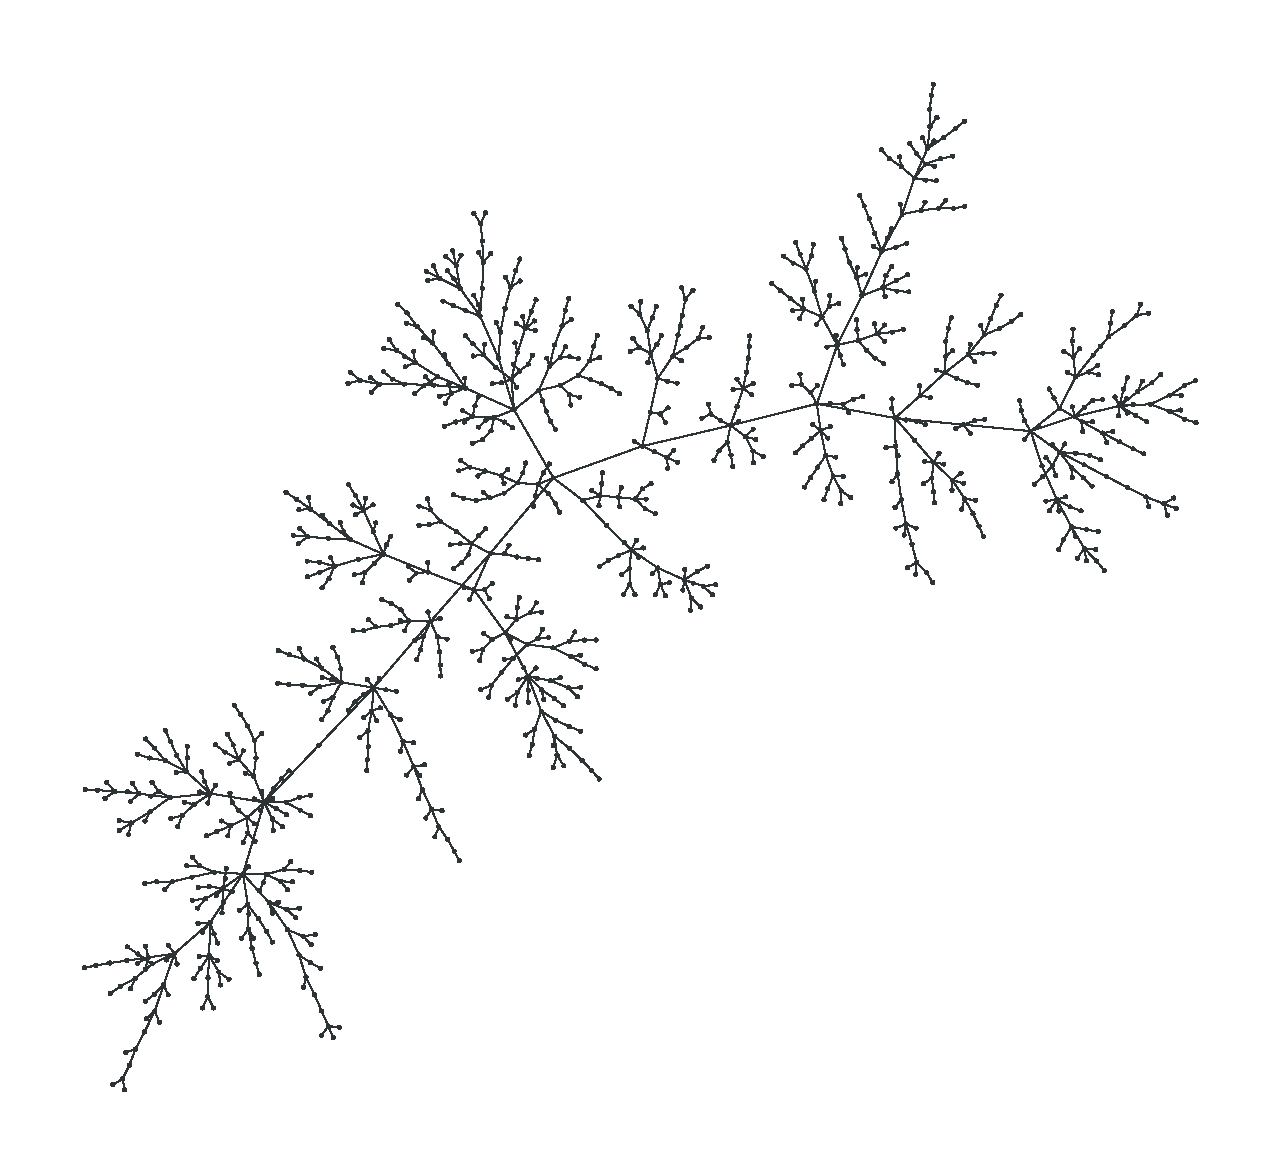
\includegraphics[width=\textwidth]{path_10.pdf}
    \caption{$S$ is a path on $10$ nodes.}
  \end{subfigure}
  \begin{subfigure}[b]{0.45\textwidth}
    \centering
    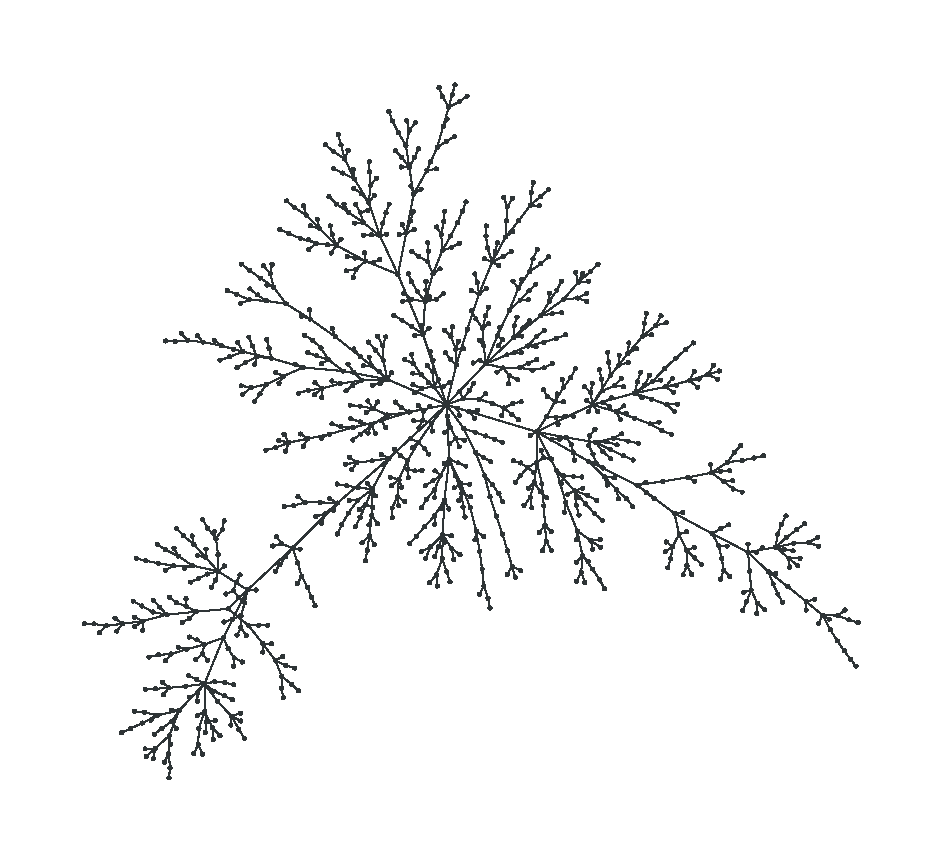
\includegraphics[width=\textwidth]{star_10.pdf}
    \caption{$S$ is a star on $10$ nodes.}
  \end{subfigure}
  \caption{One sample from $\UA(1000, S)$ for two different seeds.}
  \figlabel{ua-samples}
\end{figure}

We inductively define a distribution on labelled trees: Let
$\alpha \ge 0$, let $\UA_\alpha(k, S) = S$, and suppose that we are
given $T_{n - 1} \sim \UA_\alpha(n - 1, S)$, where
$V(T_{n - 1}) = \{u_1, \dots, u_{n - 1}\}$. Let
$T_n \sim \UA_\alpha(n, S)$ be obtained from $T_{n - 1}$ by adding a
leaf labelled $u_n$ to $T_{n - 1}$ and connecting it to a vertex
$u \in \{u_1, \dots, u_{n - 1}\}$ with probability proportional to
$\deg_{T_{n - 1}}(u)^\alpha$. The distribution $\UA_0(n, P_2)$, in
which new leaves are attached to uniformly random vertices
sequentially, is called the \emph{uniform attachment tree} or
\emph{random recursive tree}, and is sometimes denoted by
$\text{UA}(n)$ or $\text{URRT}(n)$ in the literature. The distribution
$\UA_1(n, P_2)$ is called the \emph{(linear) preferential attachment
  tree} or \emph{Barab\'{a}si-Albert model}~\cite{barabasi}, sometimes
denoted by $\text{PA}(n)$ in the literature. For $\alpha \in (0, 1)$,
$\UA_\alpha(n, P_2)$ is called the \emph{sublinear preferential
  attachment tree}, and when $\alpha > 1$, it is called the
\emph{superlinear preferential attachment tree}. For general seeds
$S$, the distributions above are said to be \emph{with seed $S$}. In
this paper, we are mostly concerned with $\UA_0(n, S)$, so we
generally omit the subscript ``0.''  Moreover, if $T \sim \UA(n, S)$
and the distribution of $T$ is understood, we avoid repeating its
distribution. See \figref{ua-samples} for a typical sample from
$\UA(n, S)$ for different choices of $S$.

The vertices of the aforementioned trees are labelled; for a (rooted
or unrooted) labelled tree $T$, let $T^\circ$ denote the isomorphism
class of $T$, \ie the operation $\circ$ ``forgets'' the labelling of
$T$. With some abuse of notation, we refer to nodes of $T^\circ$ using
their original labels in $T$. Of course, if $T \sim \UA(n, S)$ and
nothing at all is assumed about $S$, it is always possible that
$S = T$. Therefore, except if otherwise specified, we assume knowledge
of the size of the seed in trying to locate it in $T^\circ$---our main
goal is to detect $S$ in the unlabelled tree $\UA(n, S)^\circ$, given
that $|S| = k$.

In general, sets of vertices which are made to include parts of the
seed are referred to as \emph{(root-finding) vertex confidence
  sets}. We reserve the letter $H$ for functions which map unlabelled
trees to vertex confidence sets, and such functions are called
\emph{root-finding algorithms}. We also reserve the letter $K$ for the
size of vertex confidence sets.

We assume that the reader is familiar with the basics of probability
theory, including basic properties of standard random variables.  We
write $\Beta(\alpha, \beta)$ for a Beta distribution with parameters
$\alpha, \beta$, \ie the distribution supported on $[0, 1]$ with
density
\[
  f_{\alpha, \beta}(x) = \frac{1}{\mathrm{B}(\alpha, \beta)} x^{\alpha - 1} (1 - x)^{\beta - 1} ,
\]
where for $(\alpha_1, \dots, \alpha_k) \in \R^k_+$, we have
$\mathrm{B}(\alpha_1, \dots, \alpha_k) = \frac{\prod_{i = 1}^k
  \Gamma(\alpha_i)}{\Gamma(\sum_{i = 1}^k \alpha_i)}$. We write
$\Dirichlet(\alpha_1, \dots, \alpha_k)$ for the Dirichlet
distribution, which is supported on the $k$-simplex
\[
  \left\{(x_1, \dots, x_k) \colon \sum_{i = 1}^k x_i = 1 \text{ and } x_i \in [0, 1] \right\} 
\]
and which has density
\[
  f_{\alpha_1, \dots, \alpha_k}(x_1, \dots, x_k) = \frac{1}{\mathrm{B}(\alpha_1, \dots, \alpha_k)} \prod_{i = 1}^k x_i^{\alpha_i - 1} .
\]
We often make use of the following fact about the distribution of sums
of Dirichlet marginals: If
$(X_1, \dots, X_k) \sim \Dirichlet(\alpha_1, \dots, \alpha_k)$, and
$I \subseteq \{1, \dots, k\}$ is some index set, then
\[
  \sum_{i \in I} X_i \sim \Beta\left(\sum_{i \in I} \alpha_i, \sum_{i \in \{1, \dots, k\} \setminus I} \alpha_i\right) .
\]

\subsection{Acknowledgements}
The authors would like to thank the anonymous referees for their
helpful comments and suggestions. Luc Devroye is supported by NSERC
Grant A3456. Tommy Reddad is supported by an NSERC PGS D scholarship
396164433.
